\chapter{MARF Architecture}
\index{MARF!Architecture}

$Revision: 1.28 $

Before we begin, you should understand the basic
{\marf} system  architecture. Understanding how the
parts of {\marf} interact will make the follow up sections
somewhat clearer. This document presents architecture
of the {\marf} system, including the layout of the physical
directory structure, and Java packages.

Let's take a look at the general {\marf} structure in \xf{fig:arch}.
The \api{MARF} class is the central ``server'' and configuration ``placeholder'', which contains the major methods --
the core pipeline -- a typical pattern recognition process.
The figure presents basic abstract modules of the architecture.
When a developer needs to add or use a module, they derive
from the generic ones.

\begin{figure}
	\centering
	\includegraphics[angle=90,totalheight=\textheight]{../graphics/arch/arch-general.png}
	\caption{Overall Architecture}
	\label{fig:arch}
\end{figure}

The core pipeline\index{MARF!Core Pipeline} sequence diagram from an application
up until the very end result is presented in \xf{fig:pipeline}. It includes all major
participants as well as basic operations. The participants are the
modules responsible for a typical general pattern recognition pipeline.
A conceptual data-flow diagram of the pipeline is in \xf{fig:pipeline-flow}.
The grey areas indicate stub modules that are yet to be implemented.

\begin{figure}
	\centering
	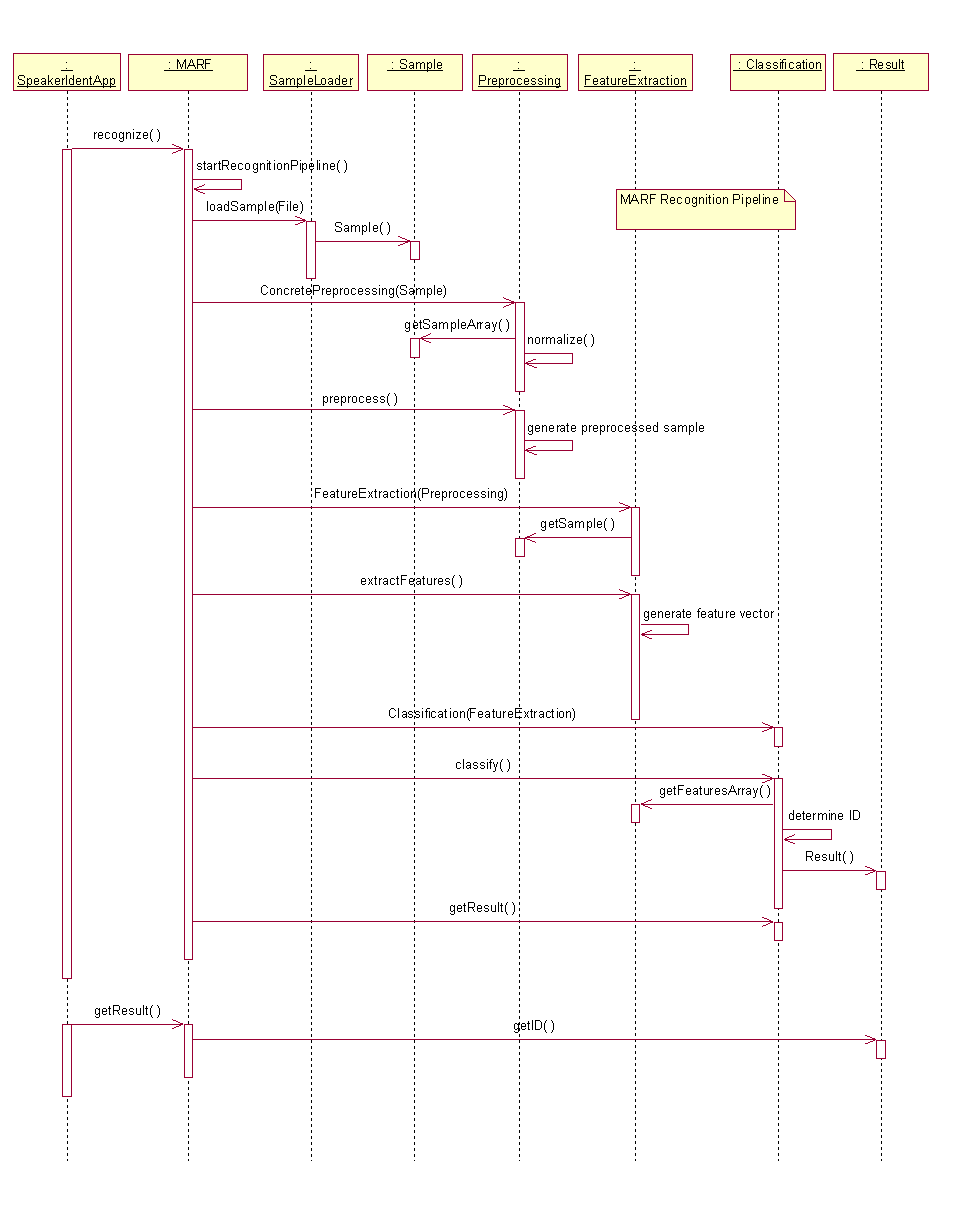
\includegraphics[angle=90,totalheight=660pt,width=550pt]{../graphics/arch/pipeline.png}
	\caption{The Core Pipeline\index{MARF!Core Pipeline} Sequence Diagram}
	\label{fig:pipeline}
\end{figure}

\begin{figure}
    \centering
    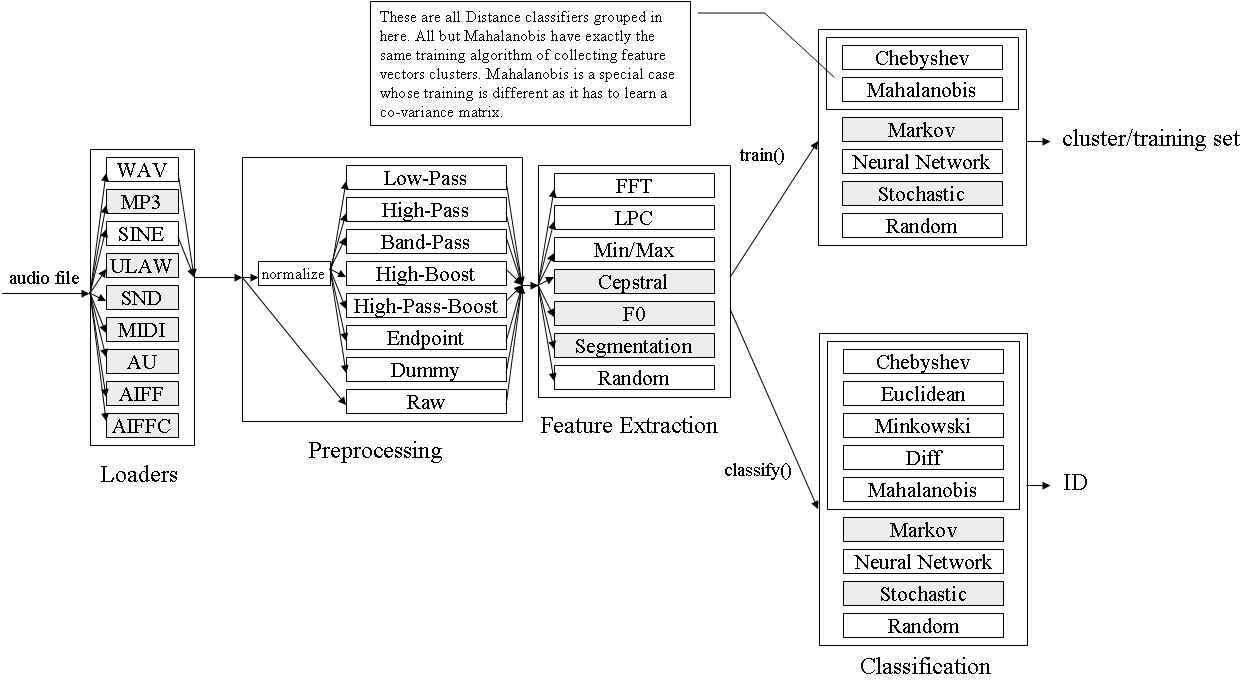
\includegraphics[width=\textwidth]{../graphics/arch/pipeline-flow.png}
    \caption{The Core Pipeline\index{MARF!Core Pipeline} Data Flow}
    \label{fig:pipeline-flow}
\end{figure}

Consequently, the framework has the mentioned basic modules,
as well as some additional entities to manage storage
and serialization of the input/output data.

\section{Application Point of View}
\index{MARF!Application Point of View}

An application, using the framework, has to choose
the concrete configuration and submodules for preprocessing,
feature extraction, and classification stages. There is an API the application
may use defined by each module or it can use them through the {\marf}.

There are two phases in {\marf}'s usage by an application:

\begin{itemize}
	\item Training, i.e. \api{train()}
	\item Recognition, i.e. \api{recognize()}
\end{itemize}

Training is performed on a virgin {\marf} installation to get
some training data in. Recognition is an actual identification process of a sample
against previously stored patterns during training.

\section{Packages and Physical Layout}
\index{MARF!Packages}

\begin{figure}
	\centering
	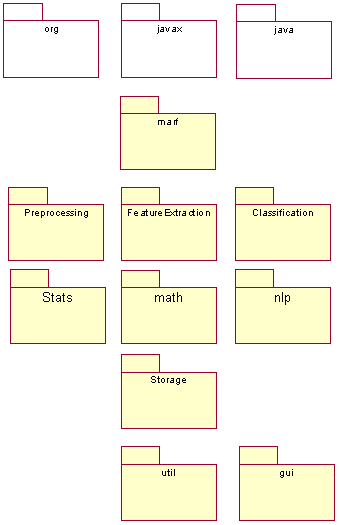
\includegraphics{../graphics/arch/packages.png}
	\caption{MARF Java Packages}
	\label{fig:packages}
\end{figure}

The Java package structure is in \xf{fig:packages}.
The following is the basic structure of {\marf}:

\vspace{15pt}
\hrule
\begin{verbatim}
marf.*

MARF.java - The MARF Server
            Supports Training and Recognition mode
            and keeps all the configuration settings.

marf.Preprocessing.* - The Preprocessing Package

/marf/Preprocessing/

   Preprocessing.java - Abstract Preprocessing Module, has to be subclassed
   PreprocessingExceotion.java

   /Endpoint/*.java   - Endpoint Filter as implementation of Preprocessing
   /Dummy/
       Dummy.java  - Normalization only
       Raw.java    - no preprocessing
   /FFTFilter/
       FFTFilter.java
       LowPassFilter.java
       HighPassFilter.java
       BandpassFilter.java - Band-pass Filter as implementation of Preprocessing
       HighFrequencyBoost.java

marf.FeatureExtraction.* - The Feature Extraction Package

/marf/FeatureExtraction/
    FeatureExtraction.java
    /FFT/FFT.java        - FFT implementation of Preprocessing
    /LPC/LPC.java        - LPC implementation of Preprocessing
    /MinMaxAmplitudes/MinMaxAmplitudes.java
    /Cepstral/*.java
    /Segmentation/*.java
    /F0/*.java

marf.Classification.* - The Classification Package

/marf/Classification/
    Classification.java
    ClassificationException.java
    /NeuralNetwork/
        NeuralNetwork.java
        Neuron.java
        Layer.java
    /Stochastic/*.java
    /Markov/*.java
    /Distance/
       Distance.java
       EuclideanDistance.java
       ChebyshevDistance.java
       MinkowskiDistance.java
       MahalonobisDistance.java
       DiffDistance.java

marf.Storage.* - The Physical Storage Management Interface

/marf/Storage/
    Sample.java
    ModuleParams.java
    TrainingSet.java
    FeatureSet.java
    Cluster.java
    Result.java
    ResultSet.java
    IStorageManager.java - Interface to be implemented by the above modules
    StorageManager.java  - The most common implementation of IStorageManager
    ISampleLoader.java   - All loaders implement this
    SampleLoader.java    - Should know how to load different sample format
    /Loaders/*.*         - WAV, MP3, ULAW, etc.
    IDatabase.java
    Database.java

marf.Stats.* - The Statistics Package meant to collect various types of stats.

/marf/Stats/
    StatsCollector.java - Time took, noise removed, patterns stored, modules available, etc.
    Ngram.java
    Observation.java
    ProbabilityTable.java
    StatisticalEstimators
    StatisticalObject.java
    WordStats.java
    /StatisticalEstimators/
        GLI.java
        KatzBackoff.java
        MLE.java
        SLI.java
        StatisticalEstimator.java
        /Smoothing/
            AddDelta.java
            AddOne.java
            GoodTuring.java
            Smoothing.java
            WittenBell.java

marf.gui.* - GUI to the graphs and configuration

/marf/gui/
    Spectrogram.java
    SpectrogramPanel.java
    WaveGrapher.java
    WaveGrapherPanel.java
    /util/
       BorderPanel.java
       ColoredStatusPanel.java
       SmartSizablePanel.java

marf.nlp.* - most of the NLP-related modules

/marf/nlp/
    Collocations/
    Parsing/
    Stemming/
    util/

marf.math.* - math-related algorithms are here

/marf/math/
    Algorithms.java
    MathException.java
    Matrix.java
    Vector.java

marf.util.* - important utility modules

/marf/util/
    Arrays.java
    BaseThread.java
    ByteUtils.java
    Debug.java
    ExpandedThreadGroup.java
    FreeVector.java
    InvalidSampleFormatException.java
    Logger.java
    MARFException.java
    Matrix.java
    NotImplementedException.java
    OptionProcessor.java
    SortComparator.java
    /comparators/
        FrequencyComparator.java
        RankComparator.java
        ResultComparator.java
\end{verbatim}
\hrule
\vspace{15pt}

\section{Current Limitations}
\index{Limiations}
\index{MARF!Current Limitaions}

Our current pipeline is maybe somewhat too rigid.
That is, there's no way to specify more than one preprocessing
to process the same sample in one pass (as of
0.3.0.2 the preprocessing modules can be chained, however, e.g.
one filter followed by another in a preprocessing pipeline).

Also, the pipeline often assumes that the whole sample is loaded before doing
anything with it, instead of sending parts of the sample a bit at a time.
Perhaps this simplifies things, but it won't allow us to deal with large
samples at the moment. However, it's not a problem for our framework
and the application because our samples are small enough and memory is cheap. Additionally,
we have streaming support already in the \api{WAVLoader} and some modules support it, but
the final conversion to streaming did not happen yet.

{\marf} provides only limited support for inter-module dependency. It is possible
to pass module-specific arguments, but problems like
number of parameters mismatch between feature extraction and classification,
and so on are not tracked.
There is also one instance of \api{ModuleParams} that exists in \api{MARF}
for now limiting combination of non-default feature extraction modules.

% EOF
